\subsection{Apparatus}

This lab is based around a single piece of equipment -- the Nuclear Magnetic Resonance spectrometer. The particular spectrometer utilized for the following experiments is shown in Figure \ref{fig:apparatus}.

\begin{figure}[H]
    \centering
    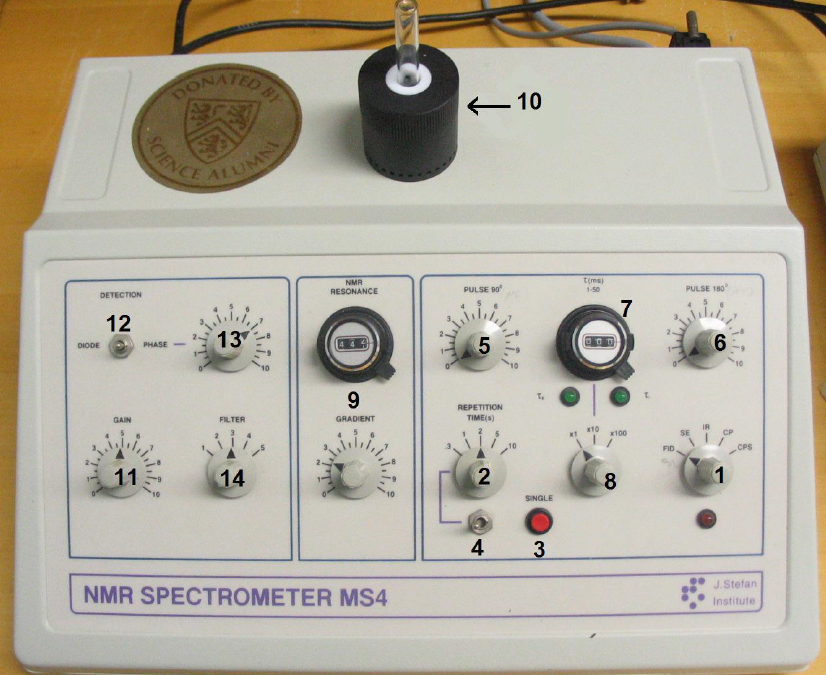
\includegraphics[width=0.66\textwidth]{figures/apparatus.PNG}
    \caption{NMR spectrometer apparatus with labelled potentiometer dials, taken from the lab manual}
    \label{fig:apparatus}
\end{figure}

The NMR spectrometer was developed in the 1950s and is commonly used to test atomic and molecular properties of samples. The spectrometers must be tuned to the particular atom which they are measuring -- setting the coil's signal equivalent to the \ref{Lfreq} of the atom to create a resonance condition (the coil is often called the radio frequency (RF) coil as most Lamour frequencies are in the RF range).  Our particular NMR spectrometer is set at a fixed frequency of 9MHz to approximately match the proton's resonance with our particular permanent magnet, but due to environmental variations this resonance frequency must be adjusted. Hence an adjustment knob is available to give a fine adjustment to the RF signal inputted ($\pm$60kHz). This is adjusted with usage of knob \#9.\\

It is possible to run many types of experiments as described in Sections \ref{sec:IR}, \ref{sec:SR} \& \ref{sec:SE}. These experiments can be chosen with the usage of knob \#1.\\

There are two knobs labelled 90$^\circ$ and 180$^\circ$ which are simply potentimeters to adjust the length of the $B_1$ pulse, hence these potentimeters directly result in affecting the overall $\vec{M}$ orientation. We note that these ``90$^\circ\:$'' and ``180$^\circ\:$'' knobs do not necessarily create the angles which are printed on the device, but simply correlate to the 90$^\circ$ and 180$^\circ$ pulses in the respective chosen experiments.\\

The ability to adjust the length of time between the experiments is also crucial for many of the experiments, and this length can be adjusted manually with usage of knobs \#7 \& 8. We note that although there is a dial which gives us the time delay, this reading is not used, instead the time delay is calculated during the data analysis as this digital measure will be more accurate and uniform across the experiments.\\

The sample is placed in a vial and ensured to be in place at the point of highest magnetic field to give the largest contrast. Also the samples are ``normalized'' which in this context means that they are set to give roughly the same voltage signal even in substances with dramatically different proton density (for example: rubber). Hence the sample is ``normalized'' with respect to voltage. The sample is placed in the holder which is labelled as \#10. \\

The left portion of the spectrometer allows for the changing of detection properties, however only the reference phase will be added to create a lock in detector to see the FID on the intrinsic $\sin(\omega t)$ signal which is known to exist from $V(t) = V_o e^{-t/T} sin(\omega t)$. This allows for the accurate detection of the envelope. This reference phase is adjusted through usage of knob \#13 and is activated through switch \#12. During the experiments, this value is always kept locked into phase sensitive detection.\\

A filter is also included in the device, however the parameters of this filter are left untouched. Instead, digital filtering is performed in post-processing data analysis. The use of this filter is discussed in Appendix \ref{append:process}.\\

All other switches and knobs are unused for this experiment. The raw signal from the detection equipment is measured on an oscilloscope, and data sets are saved for post-processing analysis and as representative results.

\subsection{Experimental Types} 

There are several types of experiments which can be completed with a NMR spectrometer, each of which depends on pushing the $\vec{M}$ into different orientations in succession. The first pulse prepares the initial magnetization, and the second pulse measures the overall magnetization change which has occurred after a waiting period, $\tau$. It is important to note that only the voltage induced due to Faraday's Law is measured. This voltage is proportional to the magnetization in the $xy$-plane: ($V \propto M_T$). So, while decay equations and relationships will be stated with respect to the $\vec{M}$, measured quantities and experimental data is provided in terms of $V$. \\

The rate of magnetization decay on the $xy$ plane is: 
\begin{equation}
    M(t) = \vec{M_o} e^{-t/T^*_2} \label{eqn:magnatization_xy}
\end{equation}

However, we note that the magnetization on the $z$-axis decays without the $T_2 \; \& \; T^B_2$ these effects only apply to the perpendicular components to $B_o$ in a sustained field. Hence the decay is modelled as:

\begin{equation}
    M(t) = \vec{M_o}- (\vec{M_o} - \vec{M(0)}) e^{-t/T_1} \label{eqn:magnatization_z}
\end{equation}

We will first look at two methods of measuring the $T_1$ quantity directly.

\subsubsection{Inversion Recovery \texorpdfstring{($\pi \rightarrow \pi/2$)}{(180 -\textgreater 90)}} \label{sec:IR}

The application of a 180$^\circ$ pulse, $M(\tau = 0) = -\vec{M_o} $. After waiting for a time $\tau$, $M(\tau = \infty) = \vec{M_o}$. From Equation \ref{eqn:magnatization_z}, we can state that:

\begin{align*}
    M(\tau) &= M_o - (M_o + M_o) e^{-t/T_1}\\
            &= M_o(1 - 2 e^{-t/T_1}) \label{eqn:IR} \numberthis
\end{align*}

During the inversion time $\tau$ (between the 180$^\circ$ and 90$^\circ$ pulses), the magnetization of the inverted sample regrows under spin lattice relaxation or thermal equilibrium toward the +$z$-direction. At the time of the $90^\circ$ pulse, push all of the $z$-component is pushed into the $xy$-plane where it can then be read. Thus sometimes, the secondary pulse is known as a ``read'' pulse. We note that the $\pi/2$ degree pulse still result in a FID which decays primarily due to spin-spin relaxation, but only the FID's peak is graphed as this shows the $z$-state after time $\tau$.

\subsubsection{Saturation Recovery \texorpdfstring{($\pi/2 \rightarrow \pi/2$)}{(90 -\textgreater 90)}} \label{sec:SR}

This scheme is similar to Inversion Recovery, but pushes the $\vec{M}$ to the xy plane instead of to $-\hat{z}$. This means: $M(\tau = 0) = 0 $ and $M(\tau = \infty) = \vec{M_o}$. Therefore:

\begin{align*}
    M(\tau) &= M_o(1 - e^{-t/T_1}) \label{eqn:SR} \numberthis
\end{align*}

This scheme is useful in certain circumstances, such as if the signal cannot be inverted as is true for quadrupolar molecules. It also has lower settle times which can lead to shorter experiments.\\

Comparing Saturation Recovery and Inversion Recovery, the Inversion Recovery method has longer recovery times and hence, is more accurate. However, in clinical settings this may cause some issues due to longer wait times in scans, while the higher resolution is generally desirable in non-clinical settings.

\subsubsection{Hahn/Spin Echo \texorpdfstring{($\pi/2 \rightarrow \pi$)}{(90 -\textgreater 180)}} \label{sec:SE}

Initially a $90^\circ$ pulse generates a transverse magnetization in the $xy$-plane and this component (which can be measured as voltage) goes as $M_T = M_o e^{\tau/T^*_2}$. Some dephasing will occur following this due to local field inhomogeneities. This dephasing is dependant on some spins processing quicker than others due to a higher local field at that location and leaving some other slower processing spins behind at the ``back of the pack''.\\

After a time $\tau$, an inverting pulse (180$^\circ$) is applied and the phases begin to dephase again. However, the regions of quicker processing spins will now be at the ``back'' and after a time 2$\tau$, both the slower and quicker regions will once again rephase once they reach the initial location. This rephased signal is known as the \textit{echo}.

\begin{figure}[H]
    \centering
    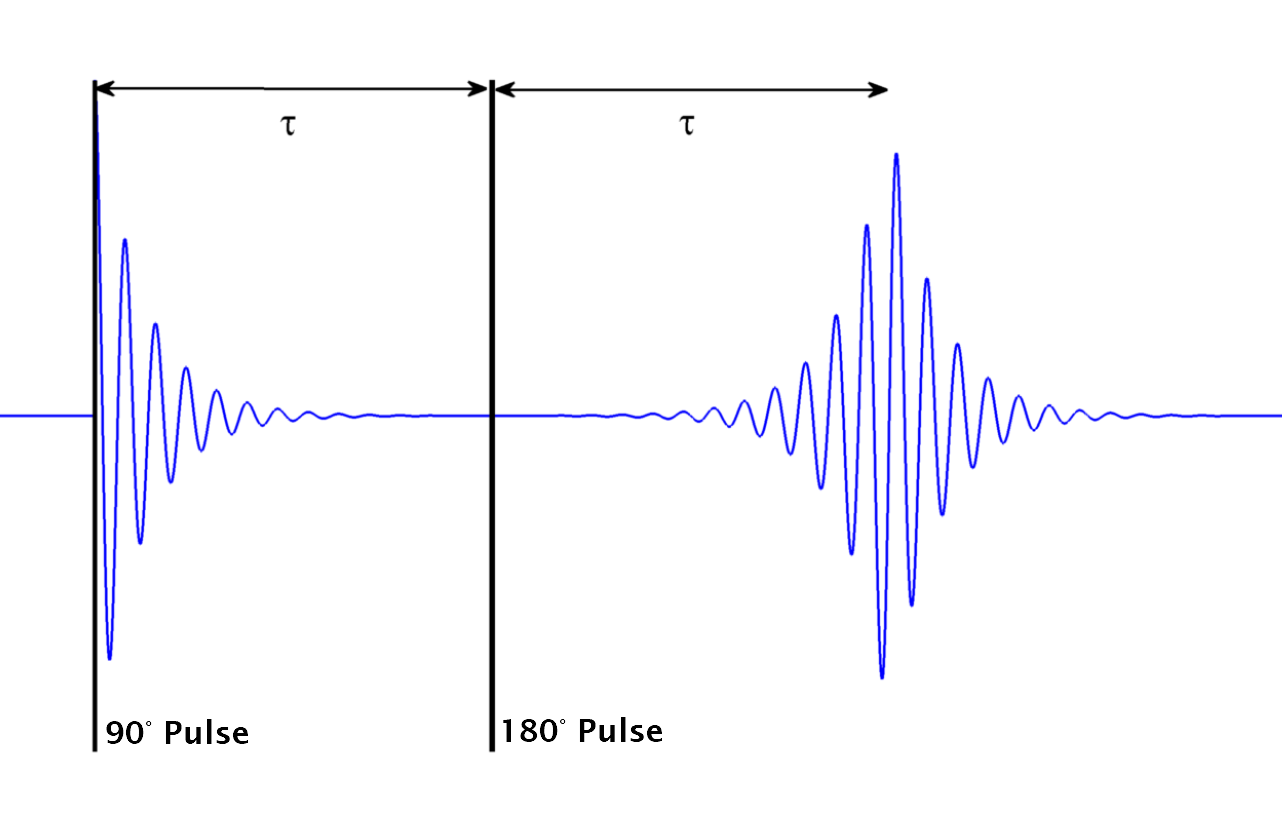
\includegraphics[width=.75\textwidth]{figures/spin_echo_ideal.png}
    \caption{An idealized simulation of a Hahn spin echo experiment with no static field inhomogeneities.}
    \label{fig:Echo}
\end{figure}

However not all of the inhomogeneities can be reversed. For paramagnet based NMR spectrometers the static field inhomogeneities dominate relaxation and the samples dynamic fields (ex. water molecules move and may experience different forces because of their alignment difference) and these effects are non-symmetric about the inversion. This means that the rephased echo will be smaller by a factor of these static field inhomogeneities, which can be modelled as, 
\[ 1/T^*_2 = 1/T_2 + \gamma \Delta B_o \numberthis \label{eqn:Hanecho} \]

In principle this experiment does not need to be completed by an inverting pulse, and these general experiments are known as spin echo experiments. However the combination of $90^\circ \; \rightarrow \; 180^\circ$ produces the maximal signal and this is known as the Hahn Echo \cite{hahn1950spin}.

\subsection{Experimental Procedure} 

During the course of the investigation six different experiments are completed. They are:

\begin{enumerate}
    \item Measurement of the Free Induction Decay (FID) of doped water at pulsed phases of $\frac{\pi}{2}$, $\pi$, $3\frac{\pi}{2}$ to observe the effects on the signal (Section \ref{B1}).
    \item Measurement of $T^*_2$ by fitting the FID curve to doped water, ethanol and rubber, all using a single $\pi/2$ pulse (Section \ref{B2}).
    \item Usage of the Saturation Recovery Sequence (\ref{sec:SR}) to find $T_1$ (Section \ref{B3}). A rough measure is found, when M($\tau$) = $M_o$/2 which can be used to approximate $T_1$. Testing is completed on all three samples.
    \item Use of Inversion Recovery Sequence (\ref{sec:IR}) to find $T_1$ (Section \ref{B4}). The decay of $\tau$ vs $M_T$ is taken at many $\tau$ and the intersection/fit can be used to accurately find $T_1$. Testing is completed on all three samples.
    \item Use of the Spin Echo Experiment (\ref{sec:SE})) to approximate the $T^B_2$ term and remove it to find an accurate measure for $T_2$ (Section \ref{B5}). Testing is completed on all three samples.
    \item Analysis of frozen (solid) doped water to explore the effects of freezing has on the FID (Section \ref{B6}). 
\end{enumerate}


\subsubsection{Finding Desired Recovery Time}

Finding the secondary pulse's recovery time is a non-trivial exercise. The following procedure describes how to calibrate the recovery times for the two pulse system.
\begin{enumerate}
    \item On settings for free induction decay (FID) experiment, adjust the repetition rate, detector phase, and first pulse length to maximize the signal for a 90 degree pulse.
    \item Measure the peak magnetization $M_0$, directly following the pulse.
    \item Switch to inversion recovery (IR) experiment.
    \item On the oscilloscope, two peaks are visible -- corresponding to the two pulses. Reduce the time delay between them and maximize the first pulse (180 degrees) such that the first peak is approximately zero and the second is maximally negative. At this point the pulse sequence is 180-$\tau$-90.
    \item If the desired pulse sequence is 180-$\tau$-90, then the parameters are set and the data can be collected (Section \ref{B4}). However, if the desired sequence is 90-$\tau$-90 (Section \ref{B3}) then approximately halve the value of the first pulse's potentiometer.
\end{enumerate}

\subsection{Data Analysis}
All data post-processing was completed using custom Matlab (Mathworks Ltd.) scripts, which are available at \url{https://github.com/tokiyoshi/460_E20_NMR.git}, along with all raw data and figures. All data was zero-shifted (such that the background is equal to zero) prior to further processing. In addition, the initial detector peak was removed from all data. This peak is caused by a ringing in the detector circuit. Filtering was performed (if needed) using a Gaussian smoothing algorithm with varying window size. Filtering was only performed if a peak value was to be automatically detected. See Appendix \ref{append:process} for discussion on data smoothing.